\documentclass{article}
\usepackage{amsmath}
\usepackage{amsfonts}
\usepackage{algorithm}
\usepackage{algpseudocode}
\usepackage{graphicx}
\usepackage{hyperref}
\hypersetup{
    colorlinks=true,
    linkcolor=blue,
    filecolor=magenta,      
    urlcolor=cyan,
}
% \usepackage[linesnumbered,boxed]{algorithm2e}


% Symbols
\newcommand{\ah}{\mc{A}_{h}}
\newcommand{\ak}{\mc{A}_{k}}
\newcommand{\ahk}{\ah \cup \ak}

\newcommand{\bin}{\set{0, 1}}
\newcommand{\binbits}[1]{\bin ^{#1}}

\newcommand{\ep}[1]{epoch_{#1}}
\newcommand{\epv}{\ep{V}}
\newcommand{\epp}{(V,\accv )}

\newcommand{\gllij}{g'_{L + 1 + i - j}}
\newcommand{\gllj}{g'_{L + 1 - j}}

\newcommand{\la}{\leftarrow}
\newcommand{\lar}{\leftarrow _{R}}

\newcommand{\mb}[1]{\mathbb{#1}}
\newcommand{\mbg}[1]{\mb{G}_{#1}}
\newcommand{\mbz}[1]{\mb{Z}_{#1}^{*}}

\newcommand{\mc}[1]{\mathcal{#1}}
\newcommand{\mch}{\mc{H}}
\newcommand{\mt}[1]{\mathtt{#1}}

\newcommand{\old}[1]{{#1}^{old}}

\newcommand{\set}[1]{\{{#1}\}}
\newcommand{\range}[1]{[{#1}]}
\newcommand{\rgp}[1]{\range{1, {#1}}}
\newcommand{\rgpl}{\rgp{l}}
\newcommand{\rgptlml}{(\rgp{2L}\backslash \set{L+1})}

\newcommand{\st}[1]{state_{#1}}
\newcommand{\stv}{\st{V}}
\newcommand{\td}[1]{\tilde{#1}}

\newcommand{\vi}{V\cup \set{i}}

\newcommand{\true}{\texttt{True}}
\newcommand{\false}{\texttt{False}}

\newcommand{\ski}{sk_{I}}
\newcommand{\pki}{pk_{I}}

\newcommand{\accv}{acc_{V}}
\newcommand{\accvi}{acc_{\vi}}

\newcommand{\cp}{C_{P}}
\newcommand{\cpp}{(\group{m_i}{i}{(\ahk )}, A, e, v)}
\newcommand{\cnr}{C_{NR}}
\newcommand{\cnrp}{(I_{A}, \sigma , c, s, \witi , g_i, g'_i, i)}
\newcommand{\cpnr}{\cp , \cnr }

\newcommand{\pk}{P_{k}}
\newcommand{\pkp}{(n, S, Z, \group{R_i}{i}{\rgpl })}
\newcommand{\pr}{P_{r}}
\newcommand{\prp}{(h, h_0, h_1, h_2, \td{h}, \hat{h}, u, pk, y, z)}
\newcommand{\pl}{\mc{P}_{1}}
\newcommand{\plp}{(c, \hat{x}_{z}, \group{ \hat{x}_{r_{i}}}{i}{\rgpl })}
\newcommand{\pkip}{(\pk , \pl , \pr )}

\newcommand{\rc}{R_{c}}
\newcommand{\rcp}{(\group{m_i}{i}{\ak }, A, e, v'', s_{e}, c')}
\newcommand{\rr}{R_{r}}
\newcommand{\rrp}{(I_{A}, \sigma , c, s'', \witi , g_{i}, g'_{i}, i)}

\newcommand{\reqp}{(U, c, \hat{v}', \group{\hat{m}_{i}}{i}{\ah},n_{1}, U_{r})}
\newcommand{\resp}{(\accv ,\mc{H}, \rc , \rr )}

\newcommand{\stp}{(V, \stpp )}
\newcommand{\stpp}{\group{g_{i}, g'_{i}}{i}{\rgptlml}}

\newcommand{\setup}{\mt{setup}}
\newcommand{\setupi}{\setup(l, L)}
\newcommand{\setupp}{(\keypair{I}, \stv , \epv )}

\newcommand{\cdt}{\mt{credential}}
\newcommand{\crreq}{\cdt _{req}}
\newcommand{\crreqp}{\crreq (\mc{S}, \ah, \group{m_i}{i}{\ah}, n_0, \mc{H}, \pki )}
\newcommand{\crres}{\cdt _{res}}
\newcommand{\crresp}{\crres (i, \old{\stv }, \mc{H}, \group{m_i}{i}{\ak }, \ski , req)}
\newcommand{\crrespp}{(res , \stv ,\epv )}
\newcommand{\crfinishp}{\cdt _{finish}(\pki , \vs , req, res)}

\newcommand{\vs}{(v', s')}

\newcommand{\proofp}{\mt{proof}(\cpnr ,\pki )}

\newcommand{\vrf}{\mt{verify}}
\newcommand{\verifyph}{\vrf _{req}(\pki , req)}
\newcommand{\verifyrnr}{\vrf _{\rr }(\accv, \mc{H}, \vs , \pki , \rr )}
\newcommand{\verifycon}{\vrf _{credential}(proof, \epv )}

\newcommand{\witi}{wit_{i}}
\newcommand{\witip}{(\sigma _{i}, u_{i}, g_{i}, w, V)}

\newcommand{\commitp}{(C, D, A, \mc{G}, \mc{W}, \mc{S}, \mc{U})}
\newcommand{\openerp}{(c, \rho , \group{m_{j}}{j}{\ak}, r, s, open, open', mult, mult', tmp, tmp', r', r'', r''')}


% Equations
\newcommand{\equivmod}[3]{#1\la #2\pmod{#3}}
\newcommand{\group}[3]{\set{#1}_{\forall #2\in #3}}
\newcommand{\keypair}[1]{sk_{#1}, pk_{#1}}
\newcommand{\keypairv}[3]{sk_{#1}\la {#2}\mbox{, }pk_{#1}\la {#3}}
\newcommand{\pairing}[2]{e(#1\mbox{, }#2)}
\newcommand{\pairingexp}[3]{\pairing{#1}{#2}^{#3}}
\newcommand{\prodi}[3]{\prod _{\forall #1\in #2}#3}
\newcommand{\randexp}[4]{#1\lar \mbz{#2}\mbox{, }#3\la #4^{#1}}
\newcommand{\randexpm}[5]{\randexp{#1}{#2}{#3}{#4}\pmod{#5}}
\newcommand{\zkp}[2]{\hat{#1}_{#2}\la \td{#1}_{#2} + c\cdot #1_{#2}}
\newcommand{\zkv}[6]{\td{#1}_{#2}\la #1_{#2}^{-#3}#4^{\hat{#5}{#6}}}



\begin{document}
\title{Cryptography of Hyperledger Indy}
\author{Kyle Huang}
\maketitle

\section{Syntax of Hyperledger Indy}
The first four steps are similar to the register operation, and the last four steps look like login.\footnote{All content refers to \href{https://hyperledger-indy.readthedocs.io/projects/hipe/en/latest/text/0109-anoncreds-protocol/README.html}{Hyperledger Indy HIPE}.}
\begin{enumerate}
\item Issuer determines a credential schema $\mc{S}$: the type of cryptographic signatures used to sign the credentials, the number $l$ of attributes in a credential, the indices $\ah \subset [1, l] = \{1, 2, ..., l\}$ of hidden attributes, the public key $P_{k}$, the non-revocation credential attribute number $l_{r}$ and non-revocation public key $P_{r}$. Then he publishes it on the ledger and announces the attribute semantics.
\item Holder retrieves the credential schema from the ledger and sets the hidden attributes.
\item Holder requests a credential from issuer. He sends hidden attributes in a blinded form to issuer and agrees on the values of known attributes $\ak \la [1, l] \backslash \ah $.
\item Issuer returns a credential pair $(C_{p}, C_{NR})$ to holder. The first credential contains the requested $l$ attributes. The second credential asserts the non-revocation status of the first one. Issuer publishes the non-revoked status of the credential on the ledger.
\item Holder approaches verifier. Verifier sends the Proof Request $\mc{E}$ to holder. The Proof Request contains the credential schema $\mc{S}_{E}$ and disclosure predicates $\mc{D}$. The predicates for attribute $m$ and value $V$ can be of form $m=V$, $m<V$, or $m>V$. Some attributes may be asserted to be the same: $m_{i}=m_{j}$.
\item Holder checks that the credential pair he holds satisfies the schema $\mc{S}_{E}$. He retrieves the non-revocation witness from the ledger.
\item Holder creates a proof $\mc{P}$ that he has a non-revoked credential satisfying the proof request $\mc{E}$ and sends it to verifier.
\item Verifier verifies the proof.
\end{enumerate}

\begin{figure}
	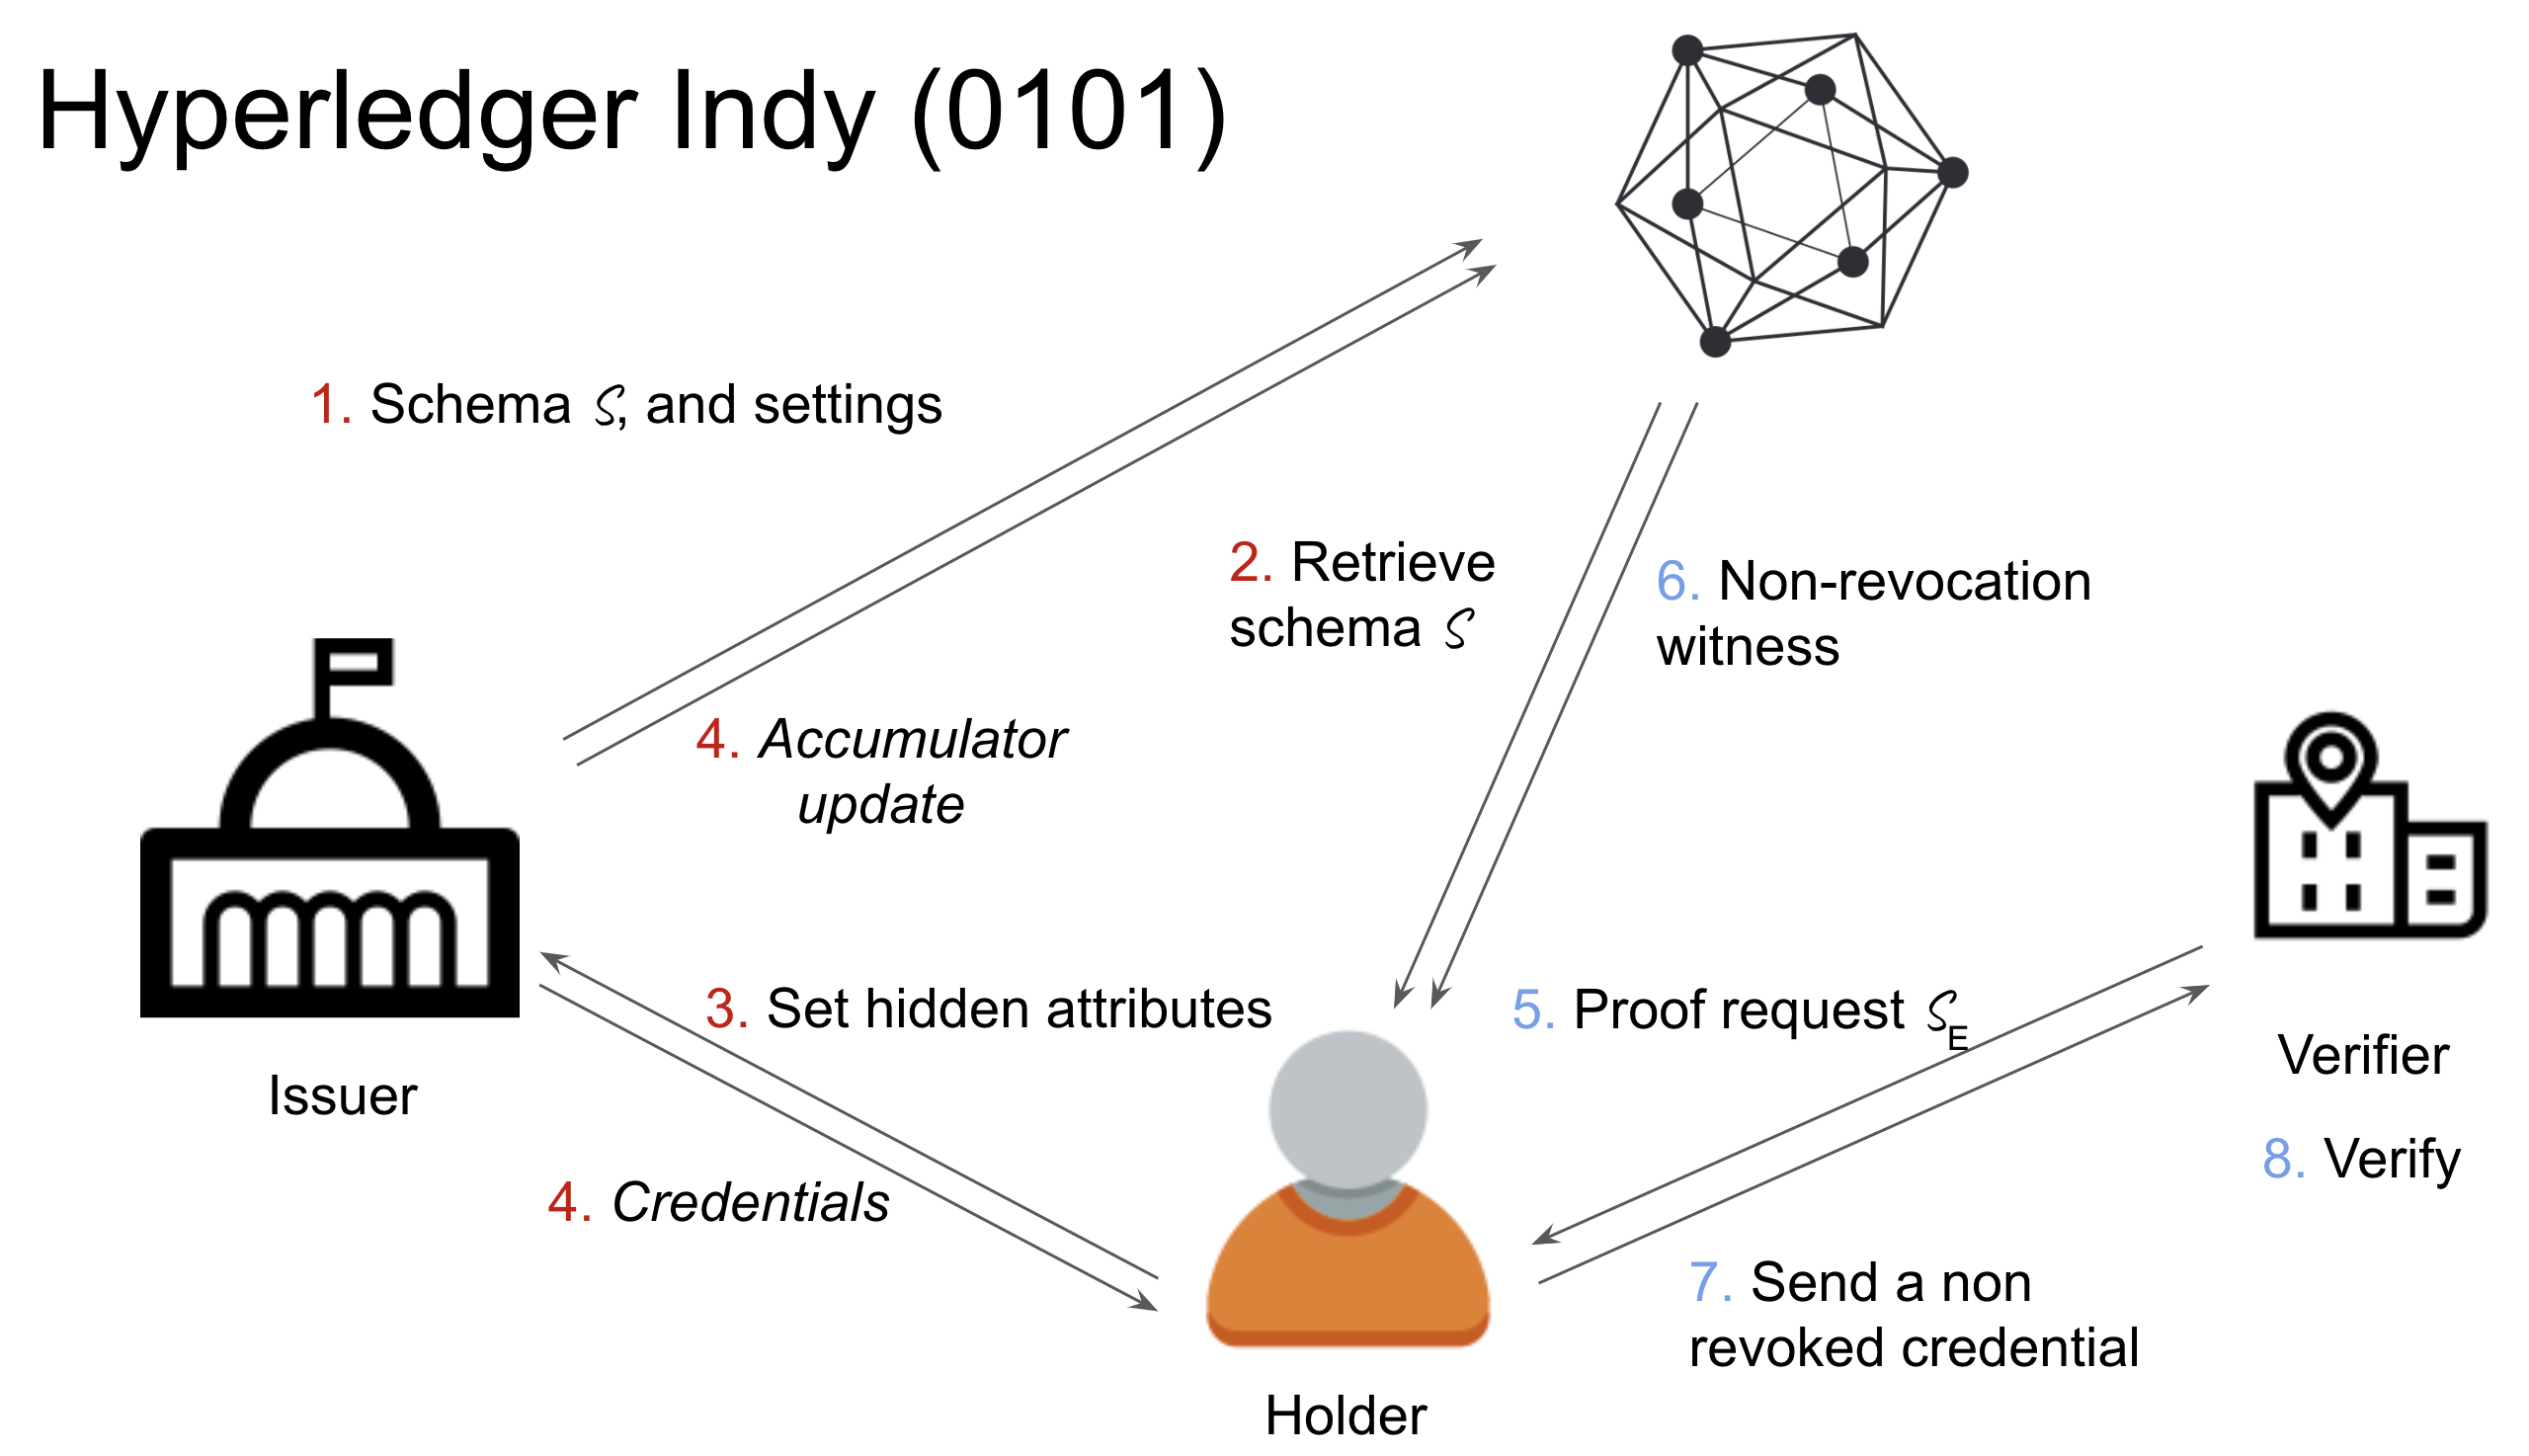
\includegraphics[width=\textwidth]{syntax.png}
	\caption{Syntax of Hyperledger Indy}
	\label{fig:indy}
\end{figure}

\begin{table}[h!]
\centering
\begin{tabular}{|c|l|} 
 \hline
 Symbol & Definition \\ \hline
 $\mc{S}$ & Schema, the empty data form with only fields. \\
 $(l, l_{r})$ & \textbf{Attributes} number and \textbf{non-revocation} credential attribute number. \\
 $L$ & The volume of a non-revocation list. \\
 $l_{a}$ & Message length for all attributes. In Sovrin, $l_{a}=256$. \\
 $(\ak, \ah)$ & The indices of \textbf{known attributes} and \textbf{hidden attributes} respectively.  \\
 & By default, $\{1, 3\}\subset \ah$ and $\{2\}\subset \ak $. \\
 $(P_{k}, P_{r})$ & Public keys of \textbf{primary credentials} and \textbf{non-revocation credentials} resp.\\
 $\mc{P}_{1}$ & Correctness proof of $P_{k}$. \\
 $(i, \mc{H})$ & The \textbf{index} and \textbf{identifier} of a holder in the issuer's view. \\
 $(\mc{V}, acc)$ & The \textbf{indices} and \textbf{accumulator} of the current non-revocation list.\\ 
 $(C_{P}, C_{NR})$ & The \textbf{primary credential} and the \textbf{non-revocation credential}.\\ \hline
\end{tabular}
\caption{Symbol table}
\label{table:symbol}
\end{table}
\clearpage
\section{Environment setup}
Issuer generates the key pair $(\keypair{k})$ and a proof $\mc{P}_{1}$ through $setup_{PC}(l)$ (Algorithm \ref{alg:pcsetup}), as well as the non-revocation key pair $(\keypair{r})$ through $setup_{NR}()$ (Algorithm \ref{alg:nrsetup}); then, he keeps $(s_{k}, s_{r})$ secret and publishes $(\mc{S}, \ah , l_{r}, P_{k}, P_{r}, \mc{P}_{1})$ to the ledger. Everyone can verify the correctness of $P_{k}$ (via proof $\mc{P}_{1}$) through $verify_{P_{k}}(l, P_{k}, \mc{P}_{1})$ (Algorithm \ref{alg:pcverify}).

\subsection{Primary Credential (CL-Signature)}

\begin{algorithm}
\caption{$setup_{PC}(l)$}
\label{alg:pcsetup}
\begin{algorithmic}
	\State $p',q'\lar \binbits{1536}$
	\Comment{$p'$ and $q'$ are prime; $|p'|=|q'|=1536$}
	\State $p\la 2p'+1$; $q\la 2q'+1$; $n\la pq$
	\Comment{$p$ and $q$ are prime}
	\State $t\lar \mbz{n}$; $\equivmod{S}{t^2}{n}$
	\State $\randexpm{x_{z}}{p'q'}{Z}{S}{n}$
	\State $\group{\randexpm{x_{r_i}}{p'q'}{R_{i}}{S}{n}}{i}{[1,l]}$
	\State $\keypairv{k}{\pk}{(p,q)}$
	\State $\randexpm{\td{x}_{z}}{p'q'}{\td{Z}}{S}{n}$
	\Comment correctness proof from here.
	\State $\group{\randexpm{\td{x}_{r_i}}{p'q'}{\td{R}_{i}}{S}{n}}{i}{[1,l]}$
	\State $c\la H_{1}(Z||\td{Z}||\group{R_i,\td{R}_i}{i}{[1,l]})$
	\Comment $H_1$ is by default SHA2-256
	\State $\zkp{x}{z}$; $\group{\zkp{x}{r_{i}}}{i}{[1,l]}$
	\State $\mc{P}_{1}\la \pl$
	\State \Return $(\keypair{k}, \mc{P}_{1})$
\end{algorithmic}
\end{algorithm}

\begin{algorithm}
\caption{$verify_{P_{k}}(l, P_{k}, \mc{P}_{1})$}
\label{alg:pcverify}
\begin{algorithmic}
	\State $\pk \la P_{k}$; $\pl \la \mc{P}_{1}$
	\State $\zkv{Z}{}{c}{S}{x}{_{z}}$; $\group{\zkv{R}{i}{c}{S}{x}{_{r_{i}}}}{i}{[1,l]}\pmod{n}$
	\State \Return $c==H_{1}(Z||\td{Z}||\group{R_i,\td{R}_i}{i}{[1,l]})$
\end{algorithmic}
\end{algorithm}

\subsection{Non-Revocation Credential}
\begin{algorithm}
\caption{$setup_{NR}()$}
\label{alg:nrsetup}
\begin{algorithmic}
	\State $\mbg{1}\times \mbg{2} \rightarrow \mbg{T}$
	\Comment pick a type-III pairing where $|\mbg{1}|=|\mbg{2}|=|\mbg{T}|=q$
	\State $g\lar \mbg{1}$; $g'\lar \mbg{2}$
	\State $h, h_0, h_1, h_2, \td{h}\lar \mbg{1}$; $u, \hat{h}\lar \mbg{2}$
	\State $\randexp{sk}{q}{pk}{g}$; $\randexp{x}{q}{y}{\hat{h}}$
	\State $\keypairv{r}{\pr}{(sk, x)}$
	\State \Return $(\keypair{r})$
\end{algorithmic}
\end{algorithm}
\subsection{CKS Accumulator}
Issuer creates a new accumulator using $setup_{Acc}(L, P_{r})$ (Algorithm \ref{alg:nracc}).
\begin{algorithm}
\caption{$setup_{Acc}(L, P_{r})$}
\label{alg:nracc}
\begin{algorithmic}
	\State $r\lar \mbz{q}$; $\group{g_{i}\la g^{r^{i}}, g'_{i}\la g'^{r^{i}}}{i}{[1, 2L] \backslash \{L + 1\}}$
	\State $z\la \pairingexp{g}{g'}{r^{L + 1}}$; $V\la \emptyset$; $acc\la 1$
	\State $\keypairv{a}{\pa }{r}$
	\State \Comment issuer publishes $(P_{a}, \mc{V})$ on the ledger with identifier $ID_{a} \la z$.
	\State \Return $(\keypair{a}, \mc{V}, acc)$
\end{algorithmic}
\end{algorithm}



\section{Credential Issuance}
Let $i<L$ and $\mc{H}$ be the index and identifier of the holder in the issuer's system, respectively. The holder acquires the schema $\mc{S}$, indices $\ah$ and public keys $(P_{k}, P_{r})$ from the ledger in addition to a random number $n_0$ and the identifier $\mc{H}$ from the issuer; then he sets the hidden attribute $\group{m_i}{i}{\ah}$. The credential issuance process is interactive, which follows: 
\begin{enumerate}
	\item The holder computes a temporary result $(\keypair{h})$ by excuting (Algorithm \ref{alg:ci1issue}) $\issuelp$; then, he keeps $s_{h}$ private and sends $(P_{h}, \group{m_i}{i}{\ak })$ to the issuer.
	\item On receiving $(P_{h}, \group{m_i}{i}{\ak })$ from the holder, the issuer firstly verifies $P_{h}$ through $\verifyph $ (Algorithm \ref{alg:phverify}). If it passes, the issuer fetches the current non-revoked indices $\mc{V}$ and accumulator $acc$ on the ledger, and runs $\issuetp$ (Algorithm \ref{alg:ci2}) to generate $(P_{PC}, P_{NR}, \mc{V}, acc)$. Finally, the issuer stores the holder’s information and index $i$ in issue’s local database; then, he updates $acc$ and $\mc{V}$ on the ledger and returns $(P_{PC}, P_{NR})$ to the holder.
	\item While receiving $(P_{PC}, P_{NR})$ from the issuer, the holder firstly runs Algorithm \ref{alg:pnrverify} to verify $P_{NR}$. If $\true \la \verifypnr $, the holder excutes Algorithm \ref{alg:ci3} $\issuethp$ to do more verifications. If all verification pass, the holder keeps the returned credential $(C_{P}, C_{NR})$.
\end{enumerate}

\begin{algorithm}
\caption{$\issuelp$}
\label{alg:ci1issue}
\begin{algorithmic}
	\State $\group{\td{m}_i\lar \binbits{593}}{i}{\ah}$
	\Comment primary credential
	\State $v'\lar \binbits{3152}$; $\td{v}'\lar \binbits{3488}$
	\State $\pk \la P_{k}$
	\State $U\la S^{v'}\prodi{i}{\ah}{R_{i}^{m_{i}}}$; $\td{U}\la S^{\td{v}'}\prodi{i}{\ah}{R_{i}^{\td{m}_{i}}}$
	\State $c = H(U||\td{U}||n_{0})$; $n_1\lar \binbits{80}$
	\State $\zkp{v}{}$; $\group{\zkp{m}{i}}{i}{\ah}$
	\State $\pr \la P_{r}$
	\Comment non-revocation credential
	\State $\randexp{s'}{q}{U_{r}}{h_{2}}$
	\State $\keypairv{h}{\ph }{\sh }$
	\State \Return $(\keypair{h})$
\end{algorithmic}
\end{algorithm}

\begin{algorithm}
\caption{$\verifyph$}
\label{alg:phverify}
\begin{algorithmic}
	\State $\pk \la P_{k}$; $\ph \la P_{h}$
	\State $\zkv{U}{}{c}{S}{v}{'}\prodi{i}{\ah}{S^{\hat{m}_{i}}R_{i}^{-c}}\pmod{n}$
	\State \Return $c == H(U||\td{U}||n_{0})$
\end{algorithmic}
\end{algorithm}

\begin{algorithm}
\caption{$\issuetp$}
\label{alg:ci2}
\begin{algorithmic}
	\State $m_{2}\la H(i||\mc{H})$
	\Comment the primary credential
	% \State \Comment store holder's information and $i$ in issue's local database
	\State $v''\la \binbits{2723}$; $e''\la \binbits{596}$
	\Comment $|v''|= 2723$, $|e| = 596$ and $e$ is prime
	\State $\pk \la P_{k}$; $\ph \la P_{h}$
	\State $Q\la Z(US^{v''}\prodi{i}{\ak}{R_{i}^{m_{i}}})^{-1}\pmod{n}$; $r\lar \mbz{p'q'}$
	\State $A\la Q^{e^{-1}\pmod{p'q'}}$; $\hat{A}\la Q^{r}\pmod{n}$
	\State $c'\la H(Q||A||\hat{A}||n_{1})$; $s_{e}\la r -c'e^{-1}$
	\State $P_{PC}\la \ppc$
	\State $s'', c\lar \mbz{q}$
	\Comment non-revocation credential
	\State $\pr \la P_{r}$, $(sk, x)\la s_{r}$
	\State $\pa \la P_{a}$, $r\la s_{a}$
	\State $\sigma \la (h_{0}h_{1}^{m_{2}}U_{r}g_{i}h_{2}^{s''})^{(x+c)^{-1}}$; $\sigma _{i} \la g'^{(sk + r^{i})^{-1}}$; $u_{i}\la u^{r^{i}}$
	\State $w\la \prodi{j}{\mc{V}}{g'_{L+1+i-j}}$; $\mc{V}\la \mc{V}\cup \{i\}$, $acc\la acc\cdot g'_{L+1-i}$
	\State $wit_{i}\la \witi $
	% \Comment publish $(acc, \mc{V})$ on the ledger
	\State $P_{NR}\la \pnr$
	\State \Return $(P_{PC}, P_{NR}, \mc{V}, acc)$
\end{algorithmic}
\end{algorithm}

\begin{algorithm}
\caption{$\verifypnr $}
\label{alg:pnrverify}
\begin{algorithmic}
	\State $\pr \la P_{r}$; $\pnr \la P_{NR}$
	\State $\witi \la wit_{i}$; $\sh \la s_{h}$
	\State $s\la s' + s''$; $m_2\la H(i||\mc{H})$
	\If{$\pairing{g_{i}}{acc}(\pairing{g}{w})^{-1}\neq z$}
		\State $\mbox{    }$\Return \false
	\ElsIf{$\pairing{pk\cdot g_{i}}{\sigma _{i}}\neq \pairing{g}{g'}$}
		\State $\mbox{    }$\Return \false
	\ElsIf{$\pairing{\sigma }{y\cdot \hat{h}^{c}}\neq \pairing{h_{0}h_{1}^{m_{2}}h_{2}^{s}\cdot g_{i}}{\hat{h}}$}
		\State $\mbox{    }$\Return \false
	\Else 
		\State $\mbox{    }$\Return \true
	\EndIf
\end{algorithmic}
\end{algorithm}

\begin{algorithm}
\caption{$\issuethp $}
\label{alg:ci3}
\begin{algorithmic}
	\State $\pk \la P_{k}$; $\ph \la P_{h}$
	\State $\ppc \la P_{PC}$; $\pnr \la P_{NR}$
	\If{$e$ is not prime OR $e\not \in [2^{596}, 2^{596} + 2^{119}]$}
		\State $\mbox{    }$\Return \textbf{null}
	\EndIf
	\State $\sh \la s_{h}$; $v\la v' + v''$; $s\la s' + s''$
	\State $Q\la Z(S^{v}\prodi{i}{(\ak \cup \ah)}{R_{i}^{m_{i}}})^{-1}\pmod{n}$
	\If{$Q\neq A^{e}$}
		\State $\mbox{    }$\Return \textbf{null}
	\EndIf
	\State $\hat{A}\la A^{c'+s_{e}\cdot e}$
	\If{$c'\neq H(Q||A||\hat{A}||n_{1})$}
		\State $\mbox{    }$\Return \textbf{null}
	\Else \State $C_{P}\la \cp$; $C_{NR}\la \cnr$
	\State \Return $(C_{P}, C_{NR})$
	\EndIf
\end{algorithmic}
\end{algorithm}

\section{Credential Revocation}
The revocation process is quite straightforward. The issuer fetches the current non-revoked indices $\mc{V}$ and accumulator $acc$ on the ledger. Then, he revokes user with index $i$ via Algorithm \ref{alg:revoke} and updates $(\mc{V}', acc')$ on the ledger after running $(\mc{V}', acc')\la revoke(\mc{V}, acc, i)$. 

\begin{algorithm}
\caption{$revoke(\mc{V}, acc, i)$}
\label{alg:revoke}
\begin{algorithmic}
	\State $\mc{V} \la \mc{V} \backslash \{i\}$
	\State $acc \la acc \cdot (g'_{L+1-i})^{-1}$
	\State \Return $(\mc{V}, acc)$
\end{algorithmic}
\end{algorithm}

\end{document}
